\documentclass[tikz,border=8pt]{standalone}
\usetikzlibrary{arrows.meta,positioning}
\begin{document}
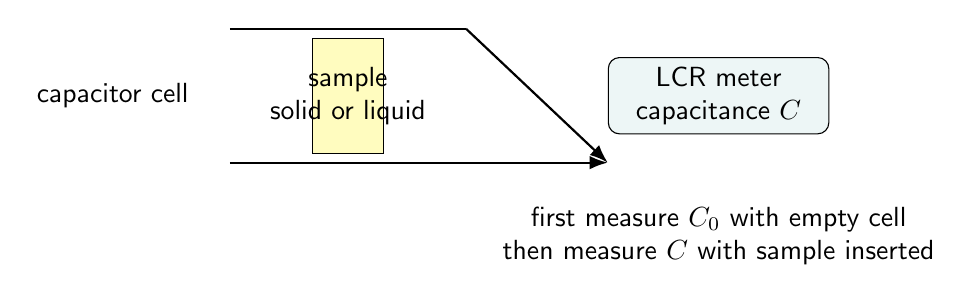
\begin{tikzpicture}[font=\sffamily,>=Latex,box/.style={draw,rounded corners,minimum height=9mm,minimum width=28mm,align=center,fill=teal!7}]
\draw[thick] (0,0)--(3,0) (0,1.7)--(3,1.7);
\draw[fill=yellow!25] (1.05,.12) rectangle (1.95,1.58);
\node[align=center] at (1.5,.85) {sample\\solid or liquid};
\node[left=4mm of {(0,.85)}] (cell) {capacitor cell};
\node[box,right=18mm of {(3,.85)}] (meter) {LCR meter\\capacitance $C$};
\draw[thick,-Latex] (3,0)--(meter.west |- 0,0);
\draw[thick,-Latex] (3,1.7)--(meter.west |- 1.7,0);
\node[below=8mm of meter,align=center] {first measure $C_0$ with empty cell\\then measure $C$ with sample inserted};
\end{tikzpicture}
\end{document}
